% Chapter 1

\chapter{Detailed Circuit Design} % Write in your own chapter title
\label{Chapter4}
\lhead{Chapter 4. \emph{Detailed Circuit Design}} % Write in your own chapter title to set the page header
The complete circuit diagram of the circuit is shown\ref{fig:1}. 
\begin{figure}[htbp]
	
		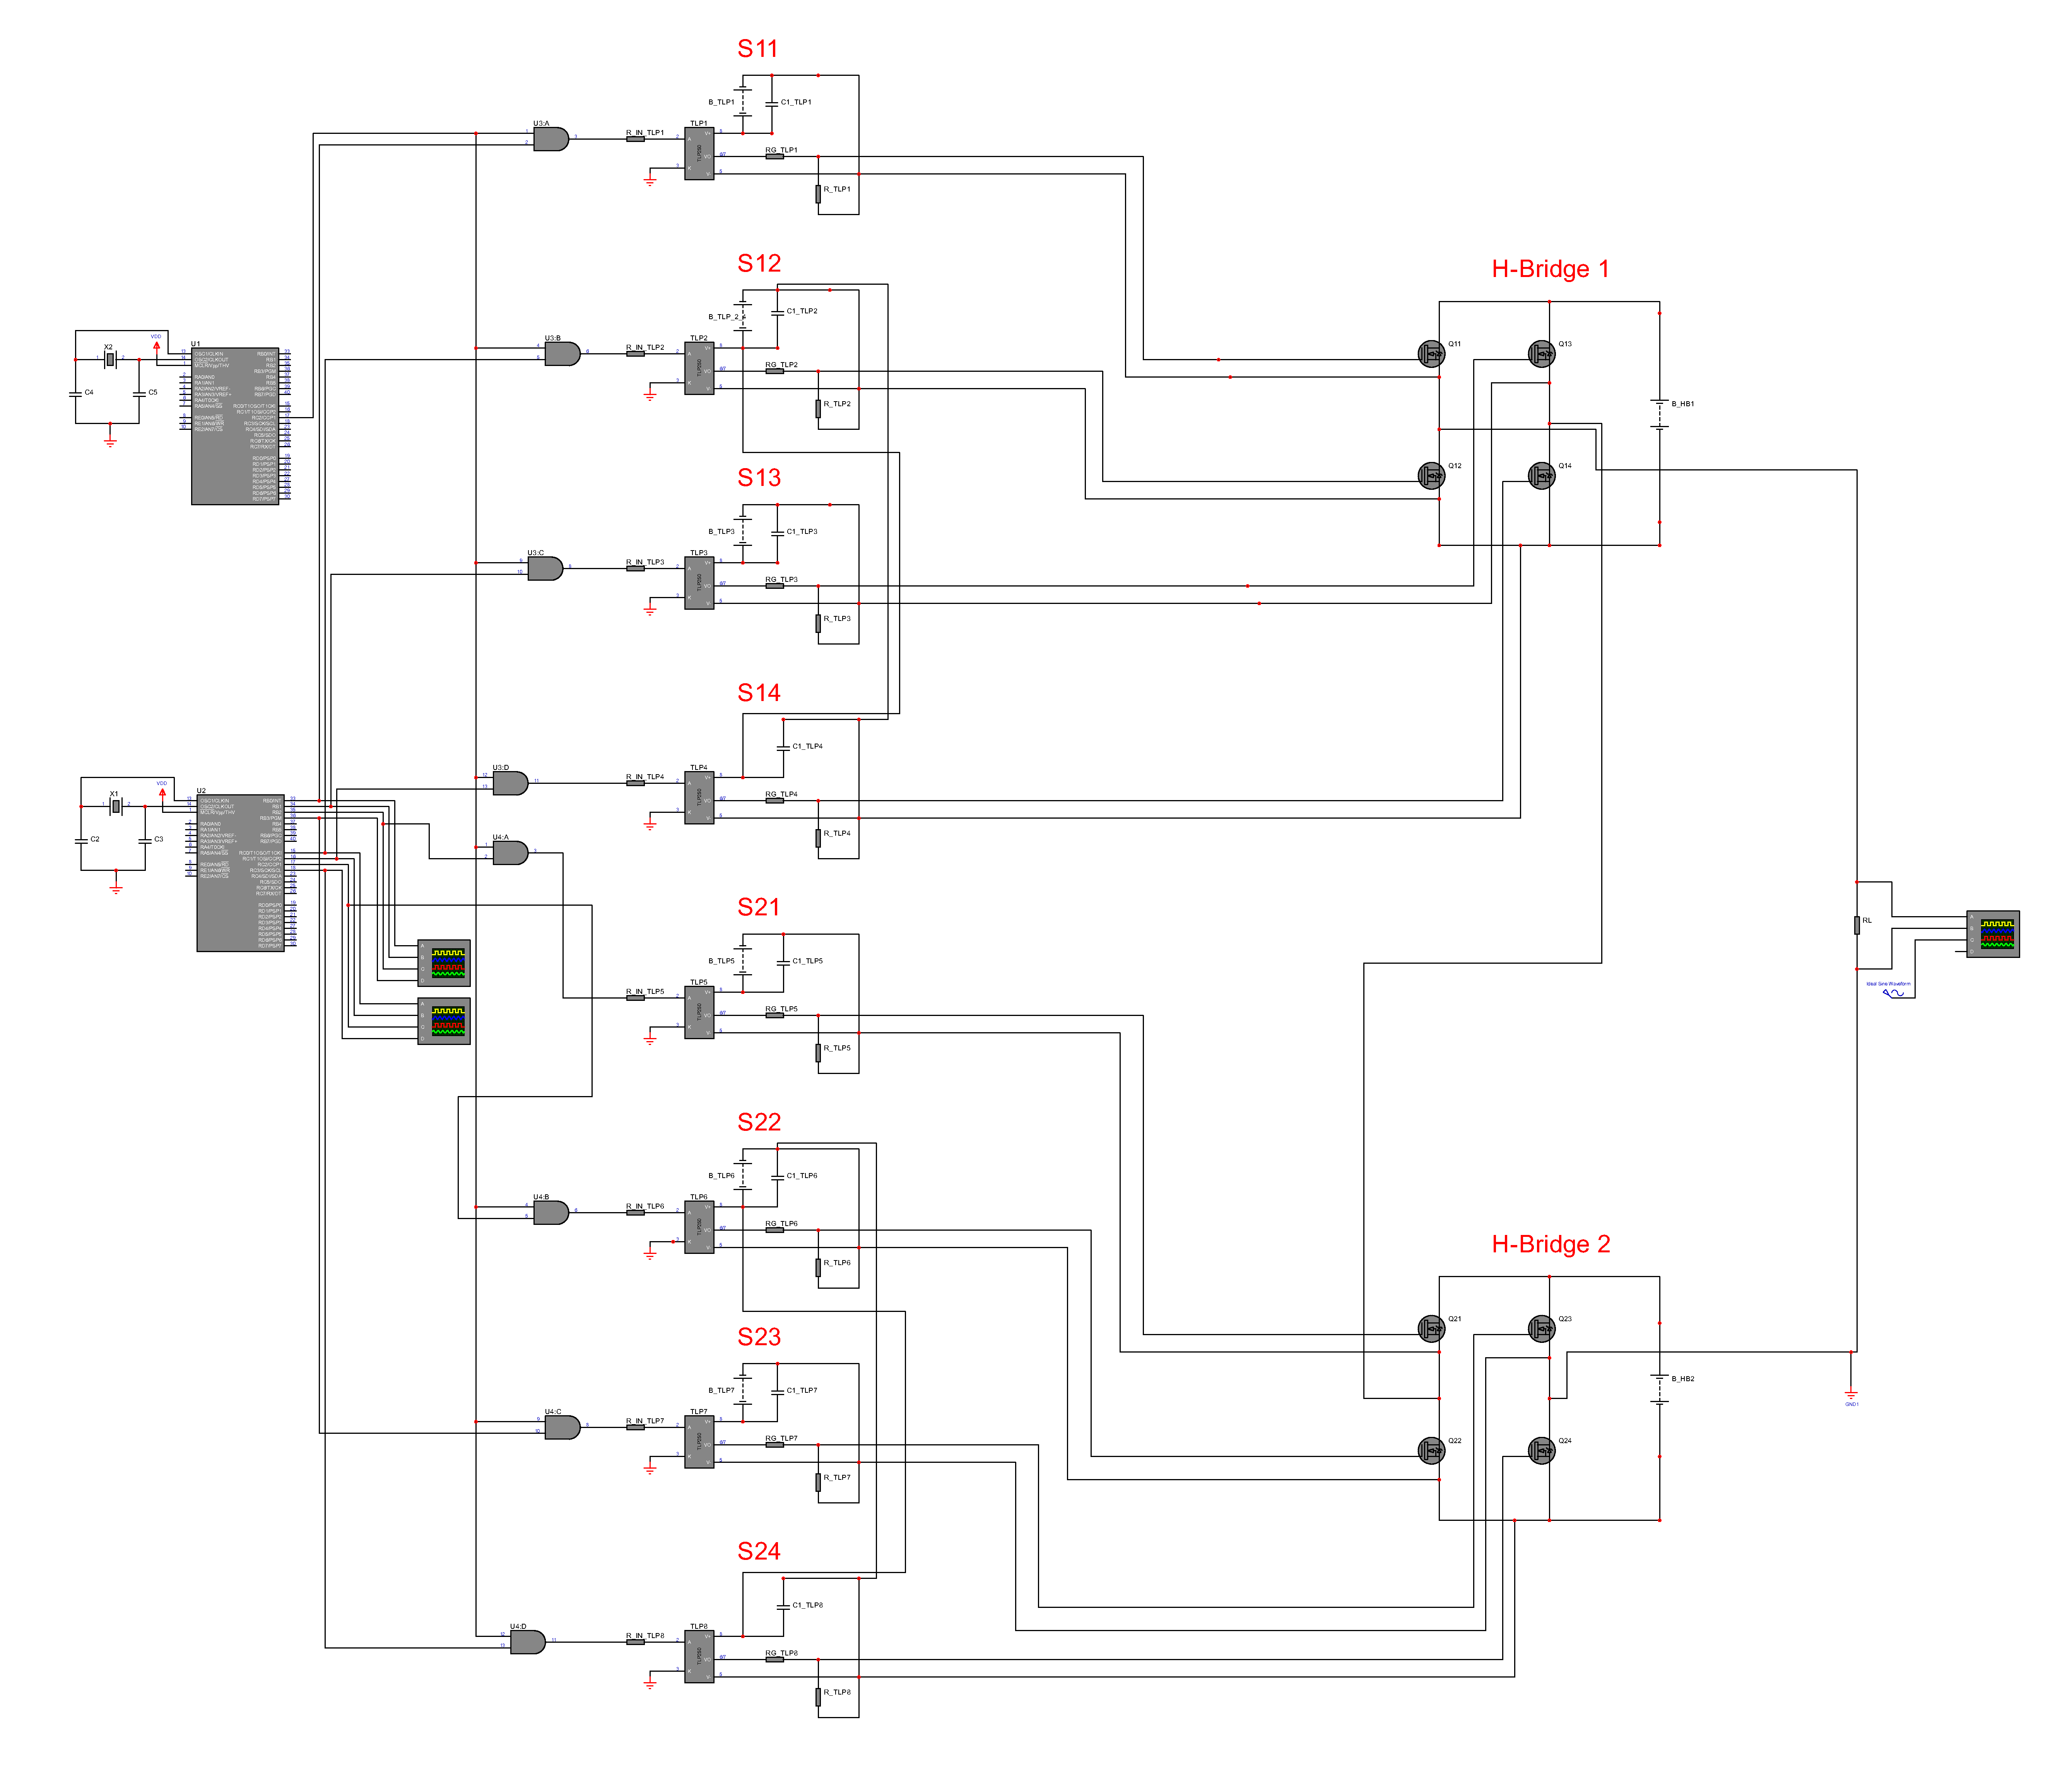
\includegraphics[width = 6in]{./Figures/Photos/circuit.pdf}
		\rule{35em}{2pt}
	\caption{Circuit for 9 Levels Voltage wave-forms}
	\label{fig:1}
\end{figure}
\newpage
The circuit\ref{fig:1} is divided into 4 main portions as:
\begin{itemize}
\item DC Supplies.
\item STM32F4x Micro-controller to apply switching.
\item Gate Triggering Circuit using Opto-coupler TLP250.
\item 2 Cascaded H-Bride Inverter.
\end{itemize}
\section{DC Supplies}
In this circuit total 8 DC supplies are used to power the circuit,6(Isolated) out of them have 15 Volts output to power the TLP 250 present in Gate triggering circuit.and the other two having outputs ratio of 1:3 vollts are used to get 9 levels output voltage waveform.Gate Drivers for ground connected Mosfets have given same supply.
\begin{figure}[htbp]
	\centering
		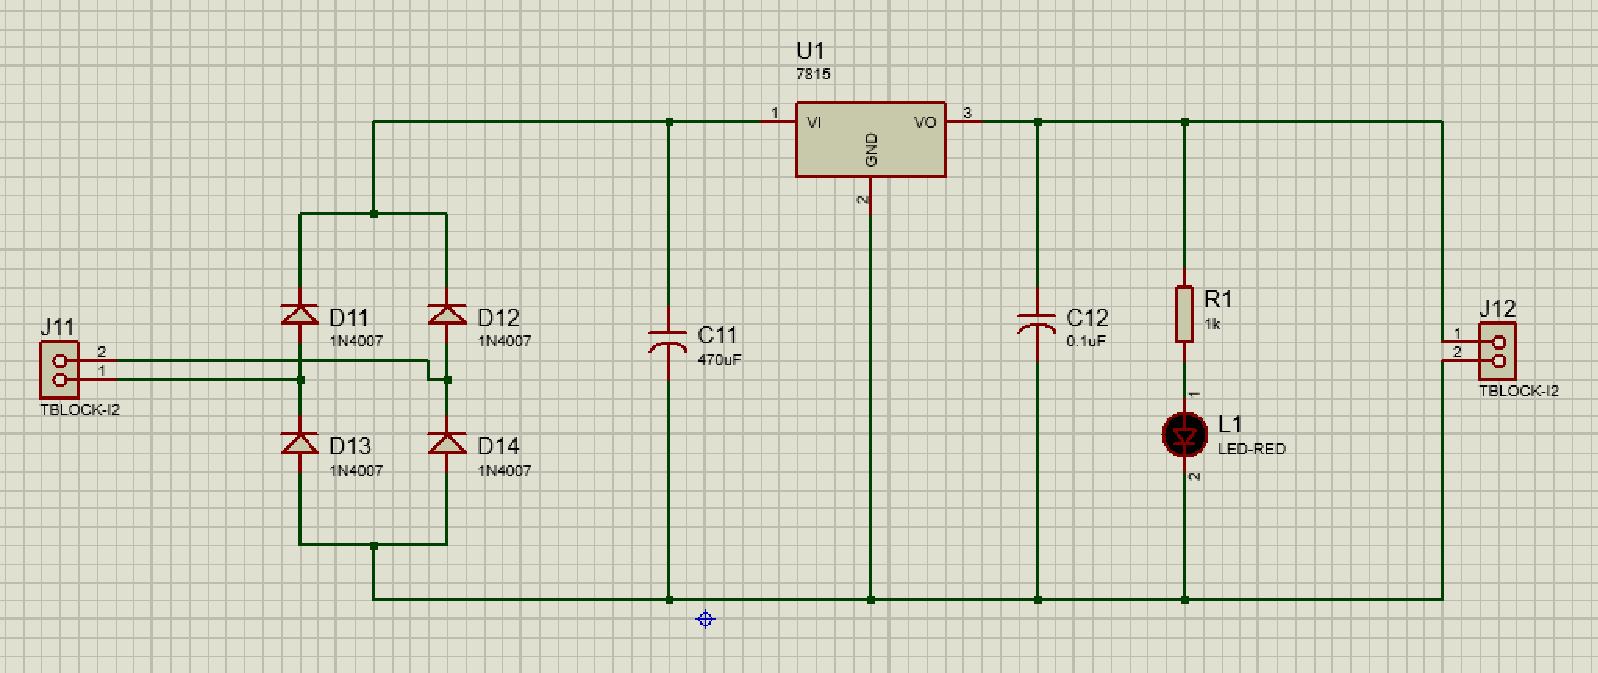
\includegraphics[width = 5in]{./Figures/ss.pdf}
		\rule{35em}{5pt}
	\caption{Circuit for Constant DC supply}
	\label{fig:2}
\end{figure}
\section{STM32F4x Microntroller}
It is a 32-bit ARM Cortex -M4 with FPU core,1-Mbyte Flash memory and 192-Kbyte RAM.
It has 6 GPIO ports and 82 I/O pins with operating voltage of 1.62-3.6v and current
rating upto 25mA. It includes 4 user LEDs and 1 user switch. The board can be power
up through USB, and it can supply 3v and 5v as external power supply.\\
This is used in this project to generate pulses at frequency of 50Hz as input of TLP250.
\section{Gate triggering circuit}	
TLP250 is 8 pin opto-coupler ic used for isolation and safety for Microcontroller also used as gate driver of switching device beause of it opto coupling ability and ability to give discharging path.
\begin{figure}[htbp]
	\centering
		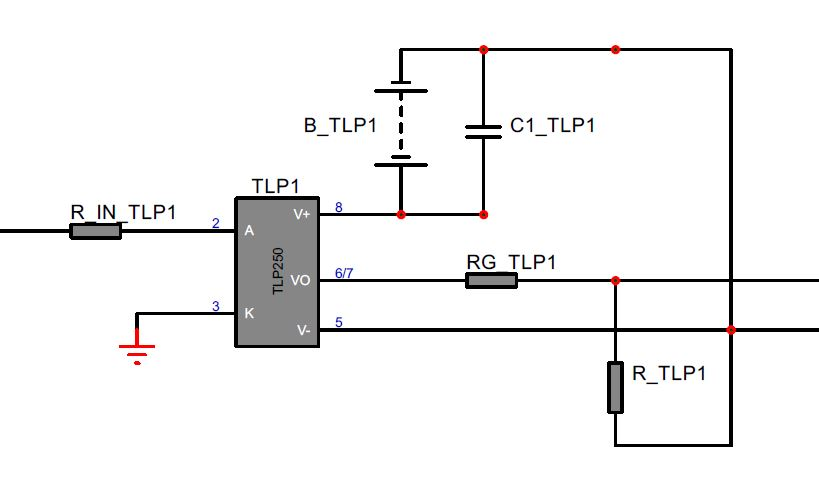
\includegraphics[width = 5in]{./Figures/Gate_driver.JPG}
		\rule{35em}{1pt}
	\caption{Circuit for TLP250}
	\label{fig:3}
\end{figure}

\begin{figure}[htbp]
	\centering
		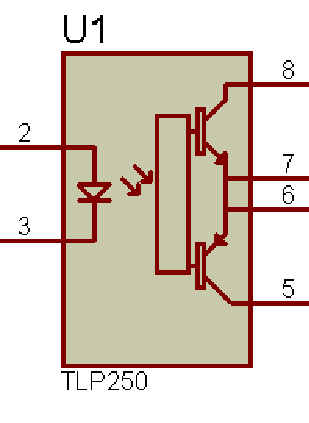
\includegraphics[width = 1.5in]{./Figures/tlp250.pdf}
		\rule{35em}{1pt}
	\caption{Inner circuit for TLP250}
	\label{fig:4}
\end{figure}
As seen from the figure\ref{fig:4} LED is connected with 2nd and 3rd pin and two BJTs are connected in series, top one to give output as $V_E$ and lower one to give discharging path.$R_in and R =1kohm $ while $R_G=10ohm$.Capacitor is of 1nF connected from pin 8 to pin 5 to stabilize the operation of the high gain linear amplifier. Failure to provide the bypassing may impair the switching property.
The pins of TLP 250 are labelled as:
\begin{itemize}
\item PIN: 2 = ANODE
\item PIN: 3 = CATHODE
\item PIN: 5 = V-/GROUND
\item PIN: 6 and 7=OUTPUT
\item PIN: 8 = V+/INPUT(15V)
\item PIN: 1 and 4 = NC
\end{itemize}
\section{H-Bridge Circuits}
There are two H-Bridge circuits used in this project[5]. By adding two H-Bridges in series so that the upper H-Bridge has DC Source = E volts and lower H-Bridge has DC Source = 3E volts, and by applying a specific switching sequence to all  switches we can obtain 9 levels in output waveform. Below the figures of all the parts are shown.

\begin{figure}[htbp]
	\centering
	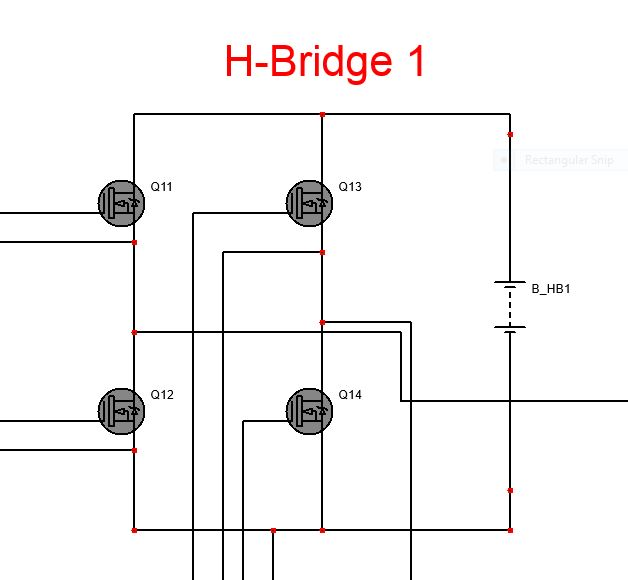
\includegraphics[width = 3.8in]{./Figures/HBridge1.JPG}
	\rule{35em}{1pt}
	\caption{H-Bridge 1 With DC Source = E volts}
	\label{fig:4}
\end{figure}
\begin{figure}[htbp]
	\centering
	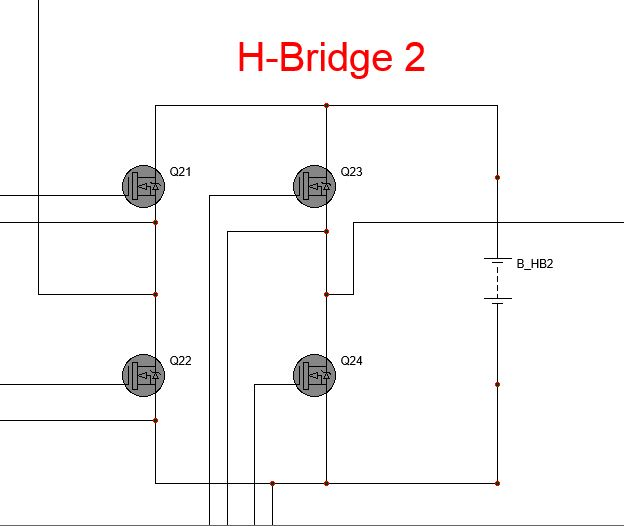
\includegraphics[width = 3.8in]{./Figures/HBridge2.JPG}
	\rule{35em}{1pt}
	\caption{H-Bridge 2 With DC Source = 3E volts}
	\label{fig:4}
\end{figure}
\begin{figure}[htbp]
	\centering
	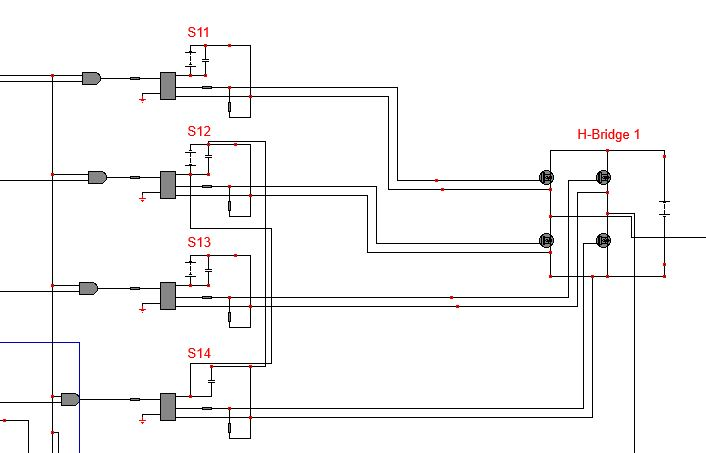
\includegraphics[width = 6in]{./Figures/C_1.JPG}
	\rule{35em}{1pt}
	\caption{H-Bridge 1 With Gate Driver Circuit}
	\label{fig:4}
\end{figure}
\begin{figure}[htbp]
	\centering
	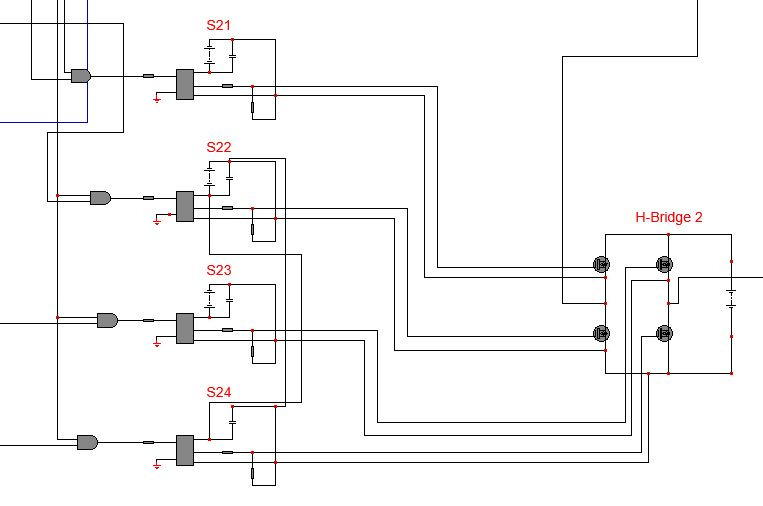
\includegraphics[width = 6in]{./Figures/C_2.JPG}
	\rule{35em}{1pt}
	\caption{H-Bridge 2 With Gate Driver Circuit}
	\label{fig:4}
\end{figure}